\section{模拟退火}
\label{sec:rs-sa}

上一节的双谷问题里，只走向更低邻居的规则停在$x=2$。这就需要回答：只维护一个状态，怎样让它有机会翻过障碍，又不至于一直乱走？\term{模拟退火}（simulated annealing，SA）的回答是：偶尔接受更差的候选，并让这种“偶尔”随时间变少。

用下山来想。一个人站在低谷里，四周都是上坡。如果他绝不上坡，就永远出不去；如果他毫不在乎坡度，就只是在地图上乱逛。合理的做法是：小坡常常愿意爬，大坡很少愿意爬，而且越到后面越不愿意爬。控制这份“愿意”的量就是温度。这个比喻到此为止：人站在山上看得到四周的坡，算法只知道它提议的那一点的代价。

\subsection{提议与接受}
\label{sec:rs-sa-accept}

一步退火由提议和接受组成。这一小节的问题是：接受规则应当怎样写，固定温度下它长期会把状态带到哪里？

\paragraph{主要思想}
一步分两半。先\textbf{提议}：从当前状态$\bm{x}$按分布$q(\bm{x},\cdot)$抽一个候选$\bm{y}$。这里设提议是对称的，即对任意$\bm{x},\bm{y}$，有$q(\bm{x},\bm{y})=q(\bm{y},\bm{x})$。

再\textbf{接受}：给定温度$T>0$，计算
\begin{equation}
 a_T(\bm{x},\bm{y})=\min\Bigl\{1,\ \exp\Bigl(-\frac{f(\bm{y})-f(\bm{x})}{T}\Bigr)\Bigr\},
 \label{eq:rs-metropolis}
\end{equation}
以概率$a_T(\bm{x},\bm{y})$移动到$\bm{y}$，否则留在$\bm{x}$。

下降或持平的提议一定被接受，上升的提议按上升量指数衰减的概率被接受。图~\ref{fig:rs-sa-acceptance}(a)画出这个函数：$T$大时曲线平缓，上坡也常被接受；$T\to0$时规则退回到只接受不上升的移动。

在双谷代价~\eqref{eq:rs-double-valley}上取$T=2$，算一次下降和一次上升。从$x=3$提议$y=2$，代价差是$-2$，接受概率为$1$。反过来，从$x=2$提议$y=3$，代价差是$+2$，接受概率为
\[
 \exp(-2/2)=\mathrm{e}^{-1}\approx0.368.
\]

上坡的代价差要除以温度才有意义。把$f$整体乘以$10$，同时把$T$乘以$10$，接受概率完全不变。所以温度的单位就是代价的单位，选温度必须看代价的尺度。

\paragraph{固定温度下的长期分布}
温度固定时，状态序列是一个马尔可夫链：下一个状态的分布只取决于当前状态。对$\bm{y}\neq\bm{x}$，一步转移的概率是
\begin{equation}
 P_T(\bm{x},\bm{y})=q(\bm{x},\bm{y})\,a_T(\bm{x},\bm{y}),
 \label{eq:rs-sa-transition}
\end{equation}
被拒绝的概率加到$P_T(\bm{x},\bm{x})$上。这个规则与下面的\term{Gibbs分布}（Gibbs distribution）紧密相关。在有限状态集合$\bm{C}$上定义
\begin{equation}
 \pi_T(\bm{x})=\frac{\exp(-f(\bm{x})/T)}{Z_T},\qquad
 Z_T=\sum_{\bm{u}\in\bm{C}}\exp(-f(\bm{u})/T).
 \label{eq:rs-gibbs}
\end{equation}
代价越低，权重越大。

\begin{theorem}[细致平衡]
\label{thm:rs-detailed-balance}
设$\bm{C}$有限，$q$对称，$T>0$。则对任意$\bm{x},\bm{y}\in\bm{C}$，
\begin{equation}
 \pi_T(\bm{x})P_T(\bm{x},\bm{y})=\pi_T(\bm{y})P_T(\bm{y},\bm{x}),
 \label{eq:rs-detailed-balance}
\end{equation}
因此$\pi_T$是转移矩阵$\bm{P}_T$的平稳分布。
\end{theorem}

\begin{proof}
$\bm{x}=\bm{y}$时两边相同。设$\bm{x}\neq\bm{y}$，不妨设$f(\bm{y})\geq f(\bm{x})$，否则交换两者的名字。这时从$\bm{y}$到$\bm{x}$是下降，$a_T(\bm{y},\bm{x})=1$，于是右边是
\[
 \pi_T(\bm{y})P_T(\bm{y},\bm{x})=\frac{\exp(-f(\bm{y})/T)}{Z_T}\,q(\bm{y},\bm{x}).
\]

从$\bm{x}$到$\bm{y}$是上升，代入式~\eqref{eq:rs-metropolis}，左边是
\[
 \begin{aligned}
 \pi_T(\bm{x})P_T(\bm{x},\bm{y})
 &=\frac{\exp(-f(\bm{x})/T)}{Z_T}\,q(\bm{x},\bm{y})\exp\Bigl(-\frac{f(\bm{y})-f(\bm{x})}{T}\Bigr)\\
 &=\frac{\exp(-f(\bm{y})/T)}{Z_T}\,q(\bm{x},\bm{y}).
 \end{aligned}
\]
由$q$的对称性，两边相等。

对式~\eqref{eq:rs-detailed-balance}关于$\bm{x}$求和，转移概率对第二个变量求和为$1$，于是
\[
 \sum_{\bm{x}}\pi_T(\bm{x})P_T(\bm{x},\bm{y})=\pi_T(\bm{y}),
\]
这正是平稳性。
\end{proof}

平稳分布存在不等于状态序列一定趋向它。若提议图连通，并且链不被周期卡住（例如某些状态有正的停留概率），状态的分布才从任何起点收敛到$\pi_T$。这一收敛结论的证明用到有限马尔可夫链的基本定理，可参考\BookChapterRef{chap:discrete-time-stochastic-processes}{卷九第3章“离散时间随机过程”}。

图~\ref{fig:rs-sa-acceptance}(b)是双谷问题的$\pi_T$。$T=2$时六号状态的概率约为$0.348$，二号状态约为$0.211$，高处的状态也有不小的份额。$T=0.5$时六号状态约为$0.850$，二号状态约为$0.115$。

\begin{BookInlineFigure}
 \centering
 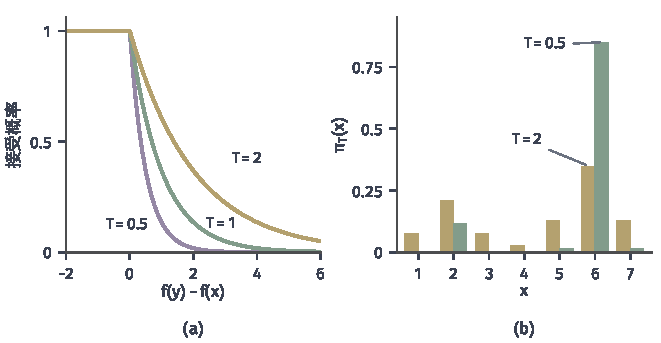
\includegraphics[width=112mm]{figures/05-optimization/05-stochastic-optimization/matplotlib/rs-sa-acceptance/figure.pdf}
 \caption{接受规则与长期分布。(a)接受概率~\eqref{eq:rs-metropolis}作为代价差的函数。(b)双谷代价~\eqref{eq:rs-double-valley}的Gibbs分布，黄色柱为$T=2$，绿色柱为$T=0.5$，温度越低，概率越集中在代价低的状态。}
 \label{fig:rs-sa-acceptance}
\end{BookInlineFigure}

温度趋于零时，$\pi_T$集中到全局最小点上。设$\bm{S}^\star$是全局最小点的集合，对任一非全局最小点$\bm{x}$和$\bm{x}^\star\in\bm{S}^\star$，比值
\[
 \frac{\pi_T(\bm{x})}{\pi_T(\bm{x}^\star)}=\exp\Bigl(-\frac{f(\bm{x})-f^\star}{T}\Bigr)\to0\qquad(T\to0^+).
\]
状态有限，所以$\pi_T(\bm{S}^\star)\to1$。这就是降温的动机：低温时的长期分布几乎全在最优解上。

问题在于“长期”。温度越低，翻越障碍越慢，走到长期分布所需的时间越长。第~\ref{sec:rs-sa-barrier}节把这件事说清楚。

\paragraph{提议不对称会怎样}
证明的最后一步用了$q$的对称性。提议不对称时，平衡关系就不再成立。看两个状态、代价相同的情形，$\pi_T=(1/2,1/2)$。

设从状态$1$总是提议$2$，而从状态$2$以$1/2$的概率提议$1$，以$1/2$的概率提议自身。代价相同，接受概率都是$1$。两状态的平稳条件是$\pi(1)\cdot1=\pi(2)\cdot\tfrac12$，于是
\[
 \pi=\Bigl(\frac13,\frac23\Bigr)\neq\Bigl(\frac12,\frac12\Bigr).
\]

要恢复目标分布，需要把提议比例放进接受概率：
\begin{equation}
 a_T(\bm{x},\bm{y})=\min\Bigl\{1,\ \exp\Bigl(-\frac{f(\bm{y})-f(\bm{x})}{T}\Bigr)\frac{q(\bm{y},\bm{x})}{q(\bm{x},\bm{y})}\Bigr\}.
 \label{eq:rs-hastings}
\end{equation}
上面的例子里，$a(1,2)=1/2$，$a(2,1)=1$，两个方向的流量都是$\pi(\cdot)\cdot\tfrac12$，$(1/2,1/2)$重新平稳。这个修正的一般讨论可参考\BookChapterRef{chap:random-sampling-integration}{卷七第14章“随机采样与积分计算”}。

\needspace{6\baselineskip}
\paragraph{变量}
下面在双谷代价上手算几步。要维护的量是：
\begin{itemize}
 \item $x^{(t)}$：当前状态，$f(x^{(t)})$是它的代价；
 \item $T^{(t)}>0$：第$t$步的温度；
 \item $x_{\mathrm{best}}$，$f_{\mathrm{best}}$：历史最好记录。
\end{itemize}

\paragraph{初始化}
选起点和初始温度，把起点记为最好记录。例中从局部低谷出发，温度每步乘以$0.9$：
\[
 x^{(0)}=2,\qquad T^{(0)}=2,\qquad T^{(t)}=2\times0.9^{t},\qquad f_{\mathrm{best}}=1.
\]
提议是等概率选左或右，超出范围时提议留在原地。

\paragraph{每轮更新}
第$t$轮依次执行以下步骤，直到用完预算。下面每一轮的提议方向和均匀随机数$u$都是事先列好的，以便逐步核对。

\begin{enumerate}
 \item 从$q(x^{(t)},\cdot)$抽候选$y$，评价$f(y)$。例中第$0$轮提议$y=1$，$f(y)=3$。
 \item 由式~\eqref{eq:rs-metropolis}计算接受概率。例中第$0$轮代价差是$2$，$T^{(0)}=2$，接受概率为$0.368$。
 \item 抽$u\sim\mathrm{U}(0,1)$，若$u<a$，令$x^{(t+1)}=y$，否则$x^{(t+1)}=x^{(t)}$。例中第$0$轮$u=0.71$，拒绝，状态仍为$2$。
 \item 若$y$可行且$f(y)<f_{\mathrm{best}}$，更新最好记录。例中第$0$轮不更新。
\end{enumerate}

表~\ref{tab:rs-sa-hand}列出前六轮。第$1$、$2$轮两次上坡都被接受，状态爬到垒顶$x=4$，代价是$5$，比记录差很多；接着第$3$、$4$轮是下坡，必然接受，第$4$轮到达$x=6$，最好记录更新为$0$。第$5$轮提议上坡到$x=7$，被拒绝。

\begin{BookInlineTable}
 \centering
 \caption{双谷代价上的前六轮，$a$是接受概率，$u$是列好的随机数。}
 \label{tab:rs-sa-hand}
 \begin{tabular}{rrrrrrrr}
  \toprule
  $t$ & $T^{(t)}$ & $x^{(t)}$ & $y$ & $f(y)-f(x^{(t)})$ & $a$ & $u$ & $f_{\mathrm{best}}$ \\
  \midrule
  $0$ & $2.000$ & $2$ & $1$ & $+2$ & $0.368$ & $0.71$ & $1$ \\
  $1$ & $1.800$ & $2$ & $3$ & $+2$ & $0.329$ & $0.25$ & $1$ \\
  $2$ & $1.620$ & $3$ & $4$ & $+2$ & $0.291$ & $0.18$ & $1$ \\
  $3$ & $1.458$ & $4$ & $5$ & $-3$ & $1$ & --- & $1$ \\
  $4$ & $1.312$ & $5$ & $6$ & $-2$ & $1$ & --- & $0$ \\
  $5$ & $1.181$ & $6$ & $7$ & $+2$ & $0.184$ & $0.62$ & $0$ \\
  \bottomrule
 \end{tabular}
\end{BookInlineTable}

最终得到$x_{\mathrm{best}}=6$，$f_{\mathrm{best}}=0$。这是特意挑选的一条幸运路径，连续爬坡两次的概率并不大，真实的成功机会要由下面的整体计算回答。

这个例子也说明了两条轨迹的区别：当前状态在第$2$轮爬到了代价$5$，比出发时差得多，而记录始终不变差。

\subsection{温度与能垒}
\label{sec:rs-sa-barrier}

温度要降到多慢，才能保证最终找到全局最小？这一小节回答这个问题，也要说明这个答案能用到什么程度。

\paragraph{能垒}
在双谷问题中，从$x=2$到代价更低的$x=6$，必须经过$x=4$。路径上的最高代价是$5$，比出发点高$4$。这个高度刻画了离开这个低谷的困难。

一般地，给定提议图和一个不是全局最小的局部低谷$\bm{x}$，考虑从$\bm{x}$到所有代价严格更低的状态的路径。路径$\bm{x}=\bm{w}_0,\bm{w}_1,\ldots,\bm{w}_k$沿提议图的边走，$f(\bm{w}_k)<f(\bm{x})$。定义\term{能垒}（energy barrier）为
\begin{equation}
 d(\bm{x})=\min_{\text{路径}}\ \max_{0\leq j\leq k}\bigl(f(\bm{w}_j)-f(\bm{x})\bigr),
 \label{eq:rs-barrier}
\end{equation}
即在所有出路中，选最省力的一条，所要爬的最大高度。全部非全局低谷的能垒中最大的一个记为$d^\star$。

双谷问题只有一个非全局低谷$x=2$。向左走不通，向右必须经过$x=4$，所以
\[
 d(2)=5-1=4,\qquad d^\star=4.
\]
图~\ref{fig:rs-barrier-depth}标出这个高度。注意能垒不等于单步的代价差：$x=2$的邻居只比它高$2$，真正要爬的是连续两步累计的$4$。

\begin{BookInlineFigure}
 \centering
 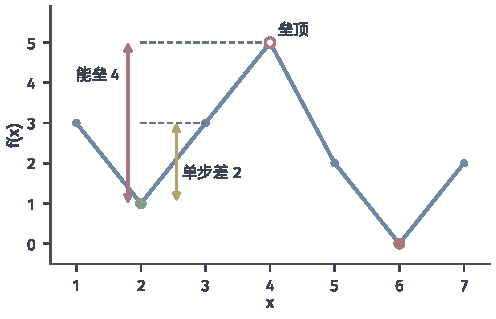
\includegraphics[width=84mm]{figures/05-optimization/05-stochastic-optimization/matplotlib/rs-barrier-depth/figure.pdf}
 \caption{双谷代价的能垒。绿点是非全局低谷$x=2$，空心红点是通往全局最小（红色实心点）必经的垒顶$x=4$。红色双箭头是能垒$d(2)=4$，黄色双箭头是一步上坡的代价差$2$。}
 \label{fig:rs-barrier-depth}
\end{BookInlineFigure}

\paragraph{对数降温的条件}
先看量级。温度为$T$时，翻过能垒$d$的那条路径大约要付出$\exp(-d/T)$的概率，所以大约要等$\exp(d/T)$步才能出去一次。$T=1$时$\mathrm{e}^4\approx55$步，$T=0.25$时已经约有$8.9\times10^{6}$步。

要让出去的机会永远不会用完，把每一步的逃逸机会加起来应当发散：
\[
 \sum_{t}\exp(-d^\star/T^{(t)})=\infty.
\]
取\term{对数降温}（logarithmic cooling）$T^{(t)}=c/\log(t+2)$，有$\exp(-d^\star/T^{(t)})=(t+2)^{-d^\star/c}$，这个级数在$c\geq d^\star$时发散，在$c<d^\star$时收敛。这就是下面定理的来历。

\begin{theorem}[对数降温下的全局收敛]
\label{thm:rs-log-cooling}
设$\bm{C}$是有限集，提议$q$对称，提议图连通，链允许原地停留。若温度取
\begin{equation}
 T^{(t)}=\frac{c}{\log(t+2)},\qquad c\geq d^\star,
 \label{eq:rs-log-cooling}
\end{equation}
则从任何起点出发，
\begin{equation}
 \lim_{t\to\infty}\mathbb{P}\bigl(\bm{x}^{(t)}\in\bm{S}^\star\bigr)=1.
 \label{eq:rs-log-cooling-limit}
\end{equation}
反之，若$0<c<d^\star$，则存在起点使这个极限不为$1$。
\end{theorem}

这一结论由Hajek于1988年给出，证明需要按代价高度逐层分析链在谷之间的转移，篇幅较长，这里不给出。下面的引理证明其中反方向的一个特殊情形，它能说明温度降得太快时发生了什么。

\begin{lemma}[降温过快时可能永远停住]
\label{lem:rs-stuck}
设$\bm{x}$的所有邻居的代价都至少比$f(\bm{x})$高$h>0$。若$T^{(t)}=c/\log(t+2)$，$0<c<h$，则从$\bm{x}$出发，状态永远不离开$\bm{x}$的概率为正。
\end{lemma}

\begin{proof}
第$t$步离开$\bm{x}$，必须接受一次上升量不小于$h$的提议，其概率不超过
\[
 \exp(-h/T^{(t)})=(t+2)^{-h/c}.
\]

记$\beta=h/c>1$。在前面各步都没有离开的条件下，第$t$步留下的概率至少是$1-(t+2)^{-\beta}$，把这些条件概率连乘，永远不离开的概率至少是
\[
 \prod_{t=0}^{\infty}\bigl(1-(t+2)^{-\beta}\bigr).
\]
由$\beta>1$，$\sum_t(t+2)^{-\beta}<\infty$，并且每个因子都大于$0$，所以这个无穷乘积大于$0$。
\end{proof}

用双谷问题具体算一次。$x=2$的两个邻居都比它高$2$，所以$h=2$。取$c=1$，提议左右各$1/2$，接受概率都是$(t+2)^{-2}$，第$t$步离开的概率恰为$(t+2)^{-2}$。于是永远留在$x=2$的概率是
\[
 \prod_{k=2}^{\infty}\Bigl(1-\frac{1}{k^2}\Bigr)=\lim_{K\to\infty}\frac{K+1}{2K}=\frac12.
\]
部分积由$(1-1/k^2)=\frac{(k-1)(k+1)}{k\cdot k}$逐项相消得到。这个算法从$x=2$出发，有一半的概率从第一步到无穷都不动。

图~\ref{fig:rs-sa-log-cooling}用转移矩阵的精确乘积算出从$x=2$出发时$x^{(t)}=6$的概率，不含抽样误差。$c=1$和$c=2$都低于$d^\star=4$，概率很快走平，到$t=2\times10^6$时分别约为$0.007$和$0.077$。$c=4$和$c=8$满足条件，概率持续上升，但到$t=2\times10^6$时也只有约$0.895$和$0.816$。

\begin{BookInlineFigure}
 \centering
 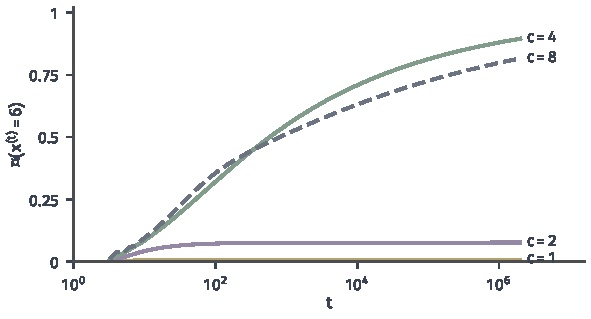
\includegraphics[width=100mm]{figures/05-optimization/05-stochastic-optimization/matplotlib/rs-sa-log-cooling/figure.pdf}
 \caption{对数降温~\eqref{eq:rs-log-cooling}下从$x=2$出发时第$t$步处于全局最小的概率，由双谷链的转移矩阵逐步相乘精确算出。$d^\star=4$，黄、紫两线的$c$小于$d^\star$，绿线取$c=4$，灰色虚线取$c=8$。横轴为对数刻度。}
 \label{fig:rs-sa-log-cooling}
\end{BookInlineFigure}

\paragraph{定理能保证什么}
这个定理的每个条件都要读准。常数$c$要覆盖能垒$d^\star$，而$d^\star$事先通常不知道。定理只对有限状态、对称连通提议成立，提议不对称或被修复过时，要重新核对。

结论是概率的极限，不是“多少步之内一定找到”。七个状态的问题，穷举只要$7$次评价，满足条件的对数降温用了两百万步仍有约一成的概率不在最优解上。$c$取得更大也不是更好：$c=8$在这个时间范围内反而不如$c=4$。

定理也不能换成任意的降温规则。按固定比例降温，$T^{(t)}=T^{(0)}\rho^t$，$0<\rho<1$，这时$\sum_t\exp(-d^\star/T^{(t)})<\infty$，定理的发散条件不满足。下一小节会看到，实际常用的正是这种规则；它能用，但不能借用上面的极限结论。

\subsection{有限预算的退火}
\label{sec:rs-sa-budget}

实际运行时，预算$B$是给定的。这一小节讨论：在$B$次评价之内，温度应当怎样安排，完整流程要包含什么？

\paragraph{三种安排}
第一种是\textbf{固定温度}，全程$T$不变，一共$B$步。第二种是\term{几何降温}（geometric cooling），每隔若干步把温度乘以比例$\rho\in(0,1)$：
\begin{equation}
 T^{[\ell]}=T^{[0]}\rho^{\ell},\qquad\ell=0,1,\ldots,K-1.
 \label{eq:rs-geometric}
\end{equation}
这里$\ell$是温度的层号，用方括号上标与迭代步区分。第三种是\textbf{分段降温}，事先列出几个温度，每个温度跑一段。

一层温度上尝试$M$次提议，共$K$层，那么一次提议就是一次评价，加上起点的一次，总评价次数是
\begin{equation}
 B=1+KM.
 \label{eq:rs-sa-budget}
\end{equation}
预算一定时，层数多则每层短，$\rho$接近$1$时降得慢。预算增加时应当把降温拉长，而不是在同样的降温后面接一段低温下的原地踏步。

\paragraph{温度的尺度}
上一小节说过，温度要和代价尺度配套。常用办法是用初始的上坡量定温度。若典型的上坡量是$\bar{\Delta}$，希望初始接受概率是$\chi_0$，那么由$\exp(-\bar{\Delta}/T^{[0]})=\chi_0$，得到
\begin{equation}
 T^{[0]}=\frac{\bar{\Delta}}{\ln(1/\chi_0)}.
 \label{eq:rs-initial-temp}
\end{equation}

双谷问题的上坡量多为$2$，取$\chi_0=0.6$，得
\[
 T^{[0]}=\frac{2}{\ln(1/0.6)}\approx3.9,
\]
可取$T^{[0]}=4$。结束温度取到上坡几乎不被接受，比如$0.1$，这时上坡量$2$的接受概率约为$2\times10^{-9}$。$\bar{\Delta}$可以先随机试若干对邻居来估计，这些试探也要记入评价次数。

提议的尺度是另一个独立的量。温度决定“接不接受”，邻域大小决定“提议走多远”。把温度调高，并不会让提议跳得更远。

\paragraph{预算内的结果}
图~\ref{fig:rs-sa-schedules}在双谷链上比较四种安排，每种安排都按预算$B$重新拉伸，并用吸收链精确计算“前$B$步内到过$x=6$”的概率。几何降温从$4$到$0.1$；分段降温依次用$4,2,1,0.5,0.25$；固定温度取$T=1$；对数降温取$c=4$。

预算为$10^4$时，几何、分段和固定温度三种安排都几乎必然到过全局最小，只有对数降温的概率约为$0.80$。对数降温在小预算时略占优势，到了大预算反而落后：它在高温停留很短，后面长时间逗留在约$0.5$的低温，翻过能垒的机会稀少。

\begin{BookInlineFigure}
 \centering
 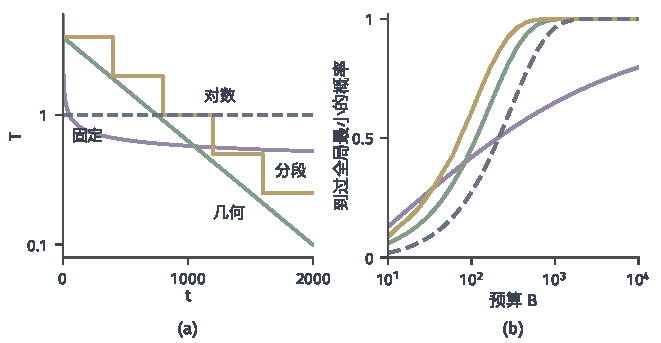
\includegraphics[width=112mm]{figures/05-optimization/05-stochastic-optimization/matplotlib/rs-sa-schedules/figure.pdf}
 \caption{双谷链上的降温安排比较。紫线为对数降温$c=4$，绿线为几何降温（$4\to0.1$），黄线为分段降温，灰色虚线为固定温度$T=1$。(a)预算$B=2000$时的温度，纵轴对数刻度。(b)预算$B$之内到过全局最小的精确概率。}
 \label{fig:rs-sa-schedules}
\end{BookInlineFigure}

这里要分清两个量。“到过”对应最好记录；“结束时停在那里”对应当前状态。预算$10^4$时，结束时处于$x=6$的概率，几何降温约为$0.79$，分段降温约为$0.75$，对数降温约为$0.71$，固定温度$T=1$约为$0.57$。固定温度下最好记录几乎一定拿到最优，当前状态却只有$\pi_1(6)\approx0.57$。

这也回答了为什么最好记录必须写进流程：不写它，固定温度下交出的当前状态有四成多的概率不是最优解。

\paragraph{完整流程}
把前面的决定合起来，一次带重启的退火这样组织。先确定预算$B$，试探代价尺度，由式~\eqref{eq:rs-initial-temp}定$T^{[0]}$，选结束温度、比例$\rho$和每层步数$M$，使总评价满足预算。

然后运行提议、接受和记录更新，每完成一层就降温。一次退火结束后，若预算还有剩余，就从新的起点重新开始，保留全局的最好记录。若单次运行成功的概率是$p$，独立重启$K$次，至少成功一次的概率是
\begin{equation}
 1-(1-p)^K.
 \label{eq:rs-restart}
\end{equation}
例如$p=0.2$，$K=5$，得到$1-0.8^5\approx0.67$。把预算切成几次短运行，单次的$p$会变小，所以切多少份要依问题试验确定。

图~\ref{fig:rs-sa-path}是二维Rastrigin函数上一次预算为$3000$的运行。高温阶段当前点在各个小坑之间跳动，代价可以高到几十；温度降低后渐渐落入一个小坑，后期几乎不再接受上坡。这次运行的最好记录为$(-0.004,0.034)$，代价约为$0.23$。

这是这一次运行得到的结果，换一个种子结果就可能不同。在有限预算下，这样的方法要按运行结果的分布评价，不能因为存在对数降温的极限定理，就说它“能收敛到全局最优”。第~\ref{sec:rs-evaluation}节回到如何评价的问题。

\begin{BookInlineFigure}
 \centering
 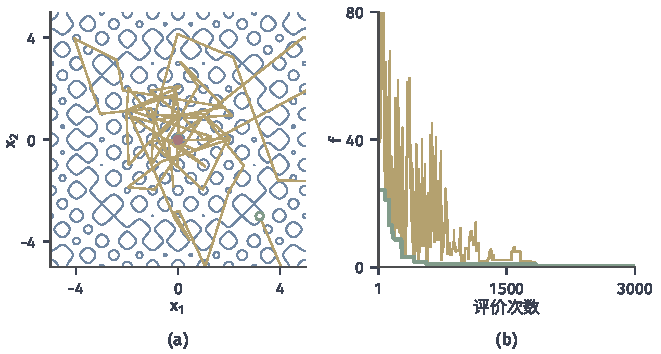
\includegraphics[width=112mm]{figures/05-optimization/05-stochastic-optimization/matplotlib/rs-sa-path/figure.pdf}
 \caption{二维Rastrigin函数~\eqref{eq:rs-rastrigin}上的一次模拟退火，高斯提议$\sigma=0.8$，温度从$25$几何下降到$0.05$，$B=3000$，种子固定。(a)蓝线是等高线，黄线是当前状态的路径（每隔$18$步取一点），空心圆是起点，绿点是最好记录，红点是全局最小点。(b)黄线是当前状态的代价，绿线是最好记录的代价。}
 \label{fig:rs-sa-path}
\end{BookInlineFigure}
